\chapter{Evaluation}
%What systems do we chose to show our evaluation on and why?
%Why are they important
%How are they different from each other?
%Why does my system selection show that our techniques are generalizable. 
Table 1 shows the sizes of the different networks we have used to evaluate our technique. They are defined by the number of inputs, layers, neurons per layer and the outputs. We test our approach on incrementally larger DNNs. Larger DNNs are networks with more layers and neurons per layer. %As mentioned previously, we have tested our approach for feed-forward neural networks that use ReLU for adding non-linearity. 

\begin{table}[h!]
	\begin{center}
		\caption{System descriptions}
		\label{tab:table1}
		\begin{tabular}{l|S|r|l}
			\textbf{} & \textbf{APS} & \textbf{HCAS} & \textbf{ACAS-Xu} \\
			%$\alpha$ & $\beta$ & $\gamma$ & $\gamma$ \\
			\hline
			\textbf{Size of the networks} &  &  &  \\
			Number of inputs &  74&   5&  5\\
			Number of hidden layers &  2&  3&  3\\
			Neurons/Layer &  8&  25 & 50 \\
			Number of outputs & 1&  5& 5\\
			\hline
			\hline
			
			%\textbf{Attacks synthesis (Avg. time in secs.)} &  &  &  \\
			%FDI attacks by perturbing 1 input &  0.01&  1000 &2700 \\
			%    FDI attacks by perturbing 2 inputs &  < 1&  2200&3600 \\
			%    FDI attacks by perturbing all inputs &  < 1&  2500& 5400 \\
			%    FDI attacks by perturbing 4 inputs  & &  & \\
			%    \hline
			%    \hline
		\end{tabular}
	\end{center}
\end{table}


\begin{table}[h!]
	%\centering
	\caption{Results Summary, Machine used: Leap 506, 8 cores}
	\label{tab:table1}
	\begin{tabular}{l|S|r|l}
		\textbf{Inputs-pert} & \textbf{Total} &  \textbf{Successful} & \textbf{Mean-Time/ } \\
		urbed/Attack &  Attacks &  Attacks &  Attack(s) \\
		\hline
		\multicolumn{4}{c}{APS}\\
		\hline
		1 &  518& 120 &  0.0015\\
		2 &  18907& 7175 &  0.002\\
		74 &  7& 7 &  0.03\\
		\hline
		\multicolumn{4}{c}{HCAS - Random}\\
		\hline
		%\textbf{HCAS}&  &   & \\
		1 &  12& 5 &  3.87\\
		2 &  12& 11 &  32.89\\
		3 &  4&  4&  41.14\\
		\hline
		\multicolumn{4}{c}{HCAS - Targeted (Partial Ordering)}\\
		\hline
		%\textbf{HCAS}&  &   & \\
		1 &  3& 1&  2.14\\
		2 &  3& 0 &  2.91\\
		3 &  1&  0&  2.74\\
		\hline
		\multicolumn{4}{c}{ACAS Xu - Random}\\
		\hline
		%\textbf{HCAS}&  &   & \\
		1 &  20& 2&  100.11\\
		2 &  40& 9& 548.72\\
		3 &  40& 12&  1452.176\\
		4 &  20&  8&  5029.58\\
		5 &  20&  2&  7228.966\\
		\hline
		\multicolumn{4}{c}{ACAS Xu- Targeted (Partial Ordering)}\\ 
		\hline
		%\textbf{HCAS}&  &   & \\
		1 &  5& 0&  297.2\\
		2 &  10& 1 &  23595.58\\
		5 &  1&  1&  8311.21\\
		\hline
		\hline
	\end{tabular}
\end{table}


\begin{table}[h!]
	\begin{center}
		\caption{Critical Inputs - APS - 1 Input perturbed at a time}
		\label{tab:table1}
		\begin{tabular}{l|S|r}
			\textbf{Output range} & \textbf{Total inputs} & \textbf{Critical Inputs}  \\
			%$\alpha$ & $\beta$ & $\gamma$ & $\gamma$ \\
			\hline
			(204 $<= Output <=$ 210) &  74&  (20, 21, 22, 23 ..)\\
			(210 $<= Output <=$ 215) &  74&   (41, 43)\\
			(200 $<= Output <=$ 203) &  74&  ( 31, 35, 36, 38, 39, 40..) \\
			(200 $<= Output <=$ 203) &  74&  (41, 42, 45, 46, 47, 48,...) \\
			%(200 <= Output <= 203) &  74& , 50, 51, 53, 54, 55, 56, 59, 60, 61, 62, 63, 64, 65, 66, 67, 68, 69, 70, 72, 73) \\
			(197 $<= Output <=$ 200) &  74&  (40, 45, 48, 49, 50....) \\
			(194 $<= Output <=$197) & 74& (40, 50, 61, 63, 66, 67...)\\
			\hline
			\hline
			
			%\textbf{Attacks synthesis (Avg. time in secs.)} &  &  &  \\
			%FDI attacks by perturbing 1 input &  0.01&  1000 &2700 \\
			%    FDI attacks by perturbing 2 inputs &  < 1&  2200&3600 \\
			%    FDI attacks by perturbing all inputs &  < 1&  2500& 5400 \\
			%    FDI attacks by perturbing 4 inputs  & &  & \\
			%    \hline
			%    \hline
		\end{tabular}
	\end{center}
\end{table}
We chose safety-critical applications for evaluating our approach. Our first application was inspired by the open-source system called openAPS.
Dutta et al. \cite{10.1007/978-3-319-99429-1_11} proposed a DNN for APS that takes in 74 inputs by discretizing time. This is a data-driven model and hence, finding attacks in such modeling is particularly interesting because it allows us to understand changing what values at a particular time will cause a change in the final output. We demonstrate this in more detail below. The second and third systems are modeling a collision avoidance (CA) system. The researchers proposed ACAS Xu standards that are tailored for threat CA logic and horizontal logic \cite{7778055}. There are 45 DNNs that together make up the collision avoidance system \cite{Julian_2019}.  Julian et al. proposed a DNN compression for ACAS by representing large data tables in the form of DNNs. The ACAS Xu dataset is currently proprietary and hence we did not have access to it. Our tool requires only the trained model to synthesize FDI attacks. HCAS is an open-source model created for collision avoidance. The reason we test our approach on both ACAS and HCAS is that the sizes of these systems are different; this choice was made to determine how well our method scales. The cost functions evaluated are the same in both cases. We decided three unique DNN models was a reasonable choice for evaluation.

\section{APS}
%The APS model designed by Kushner et al. \cite{Dutta_Others__2018__Robust}\smi{add space here}is a data-driven model. The goal of the model is to predict future blood glucose values for the patients.
APS is the running example that we have used throughout the paper. 
APS model predicts the glucose value at a "lookahead" time $t + T$, using the history of the past $N$ glucose values with a step size of $h$. The step size implies that the data is recorded after every $h$ seconds from the starting time. The inputs contain the past insulin values and glucose values by keeping the step size $h$ as 5 and the neural network builds the mapping between input and output values. It is a network with two hidden layers (with 8 neurons per layer), 74 inputs and one output that predicts the future glucose values as shown in Figure 1. 

%Attacks in the APS system.
Using our modeling we can successfully synthesize attacks in less than a minute.
%The experiments that we conduct
We incrementally conduct attack synthesis. 
\section{Attacks}
The goal is to minimize the input perturbations such that the output is perturbed by amounts such that it remains between the user-specified lower and the upper bounds. The reason we evaluate for such attacks is that in APS, even small deviations from the original outputs can cause damage. Injecting more than the required amounts even if within the bounds is undesirable.

%Randomly changing inputs can trigger alarms in the system because it will raise the levels above the bounds enforced by specifications. We want to perturb the inputs in a stealthy way. The stealthiness is induced by finding the exact perturbations and to find those exact perturbations we need \tool. Brute force would require to search through the entire search space. We model the attack by including a $delta$ function in the inputs. 
To locate the critical inputs we first perturb the inputs one at a time to induce small perturbations in the outputs as shown in Table II under the APS section. We find that for different ranges of outputs, the critical inputs vary as shown in Table III. We have included the critical inputs when we perturb only one input at a time since these are the most useful from an attackers' perspective. 

%, For example, we find that when we perturb one input for an output range of 194-197, changing any one of these (40, 50, 61, 63, 66, 67, 72, 73) inputs by certain amounts will result in a successful  FDI \attack. Due to space reasons, we provide a summary of all combinations of attacks in Table II for APS. 
%Along with the critical inputs, we also obtain the perturbations that will lead to an output deviation. 
%Further we try 

%We observe that it is feasible to find one input perturbation that can cause output perturbations without getting detected. We find every attack for APS within seconds. We test out our approach by perturbing specific inputs at a time instead of randomly finding attacks. 

%We generate attacks by keeping all inputs constant but one to observe the above phenomenon. We keep all inputs constant but two in the next set of the experiment to understand if it is easier to find such attacks as compared to finding only one input perturbation and in the process, we are successfully able to locate the critical inputs.  




%% Explain the results in this paragraph                                                                                        




%\section{FDI attack 2}
%In our next set of attacks we maximize the output deviation and minimize the input deviations. We do so to cause the maximum damage possible to a patient by perturbing inputs within bounds yet we want it to perturb by maximum amounts within those bounds. As shown in Table 2  in the lower half we conduct a similar analysis by keeping everything constant but perturbing on 1, 2 and then finally all inputs together. We conduct these experiments to show that our technique is capable of identifying one critical input and also a set of critical inputs that can cause output deviations. 

\section{ACAS Xu and HCAS}
We test our approach on two other available systems that are collision avoidance (CA) as explained in the above section. The ACAS Xu and HCAS are different in terms of their architectures and parameters as described in Table 1. Apart from the difference between the weights, bias and the number of layers, the datasets used to produce the two are also quite different.  

%We conduct two random and targeted \attack \smi{this is singular but should perhaps be plural; good idea to skim the rest of the paper where \attack is used} in these systems, to understand how the systems\smi{this sentence is incomplete}
The ACAS Xu is designed to model a large lookup table that maps the sensor readings to the advisories. There are five sensor readings:  Distance from ownship to intruder, Angle to the intruder relative to ownship heading direction, Header angle to intruder relative to ownship heading direction, speed of ownship and speed of intruder. The geometry of the ACAS Xu is shown in Figure 6. The outputs represent five different possible advisories: clear-of-conflict (COC), weak right, strong right, weak left, and strong right. Based on the inputs, the one with the least value is the advisory that is going to be the action to be taken.  We conduct two types of FDI attacks here: targeted and random. The reason we conduct these two types of attacks is that we want to understand the difficulty of synthesizing these attacks. In targeted attacks, we have to specifically choose an output that not only has to be minimized but has to have the smallest values of the five possible outcomes. The Horizontal CAS(HCAS) system works in a similar way except that it takes in three inputs instead of five. %Also, as shown in Table 1, the parameters are different for ACAS Xu and HCAS. 
The reason it takes Gurobi more time to solve the constraints in targeted attacks as compared to random attacks is the stricter ordering on the outputs.

\begin{figure}
	\centering
	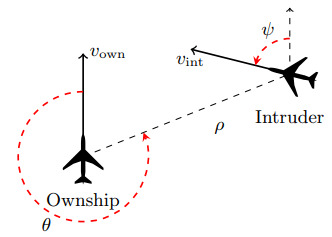
\includegraphics[width=0.7\linewidth]{Images/ACASXugeometry}
	\caption[ACAS Xu]{ACAS Xu geometry}
	\label{fig:acasxugeometry}
\end{figure}

%Explain about the normalization layer
The one feature about these systems that are different from the previous system which is the APS is that these systems consist of inputs and outputs normalization. These normalizations are used to place bounds on how much the inputs can be perturbed by. To accommodate the normalization layer, we introduce certain heuristics that are deep network specific. %The normalization depends on the conditions that are introduced by the neural network.

\section{Targeted attack} 
In the first attack, we minimize the input perturbations by keeping all but $1$, $2$ and $n$ inputs constant in the three sets of experiments that we conduct as shown in Table II for HCAS and ACAS Xu. We minimize the input perturbations but the goal is not to maximize the outputs in this case but to change the values of the inputs in a way that the output changes from slightly left to slightly right or changes from slightly right to strictly left. To find the input perturbations for such attacks the modeling has to be more precise.

For example: Consider a set of five inputs for which the output is slightly left. The output is slightly left implies that out of the five output values in the DNN, the least value is of the output that signifies slightly left which is the Output four. The network is trained in a way such that the least value signifies the output that should be taken next. Our goal is to change the output in a way such that the minimum value changes from slightly left to slightly right. To model this, we first add a delta value to the inputs as in our previous evaluation. Our goal is to minimize the deltas values, however, our goal is to not minimize or maximize the outputs but change the values of the outputs such that the smallest output is switched with the output we want it to have. To do so, we add constraints that specify that in the modeling $Output 4 > Output 5$. This would mean that the $Output 4$ now has a greater value than $Output 5$ and hence, ideally we would consider that the constraint modeling is solved. However, since this is a targeted attack we want the value of $Output 5$ to be minimized with respect to all the other outputs and not only $Output 4$. To do so, we have to add more constraints to specify that Output 5 should be the smallest among all the other output values.

\begin{figure}
	\centering
	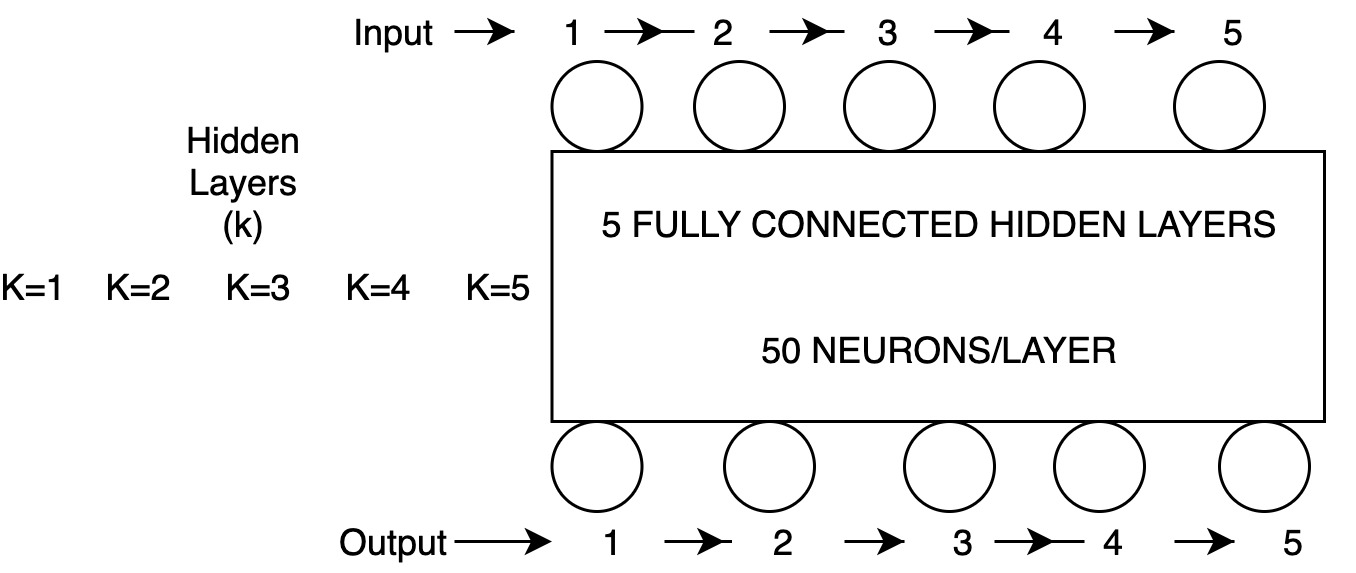
\includegraphics[width=0.7\linewidth]{Images/ACASXuDNN}
	\caption[ACAS Xu DNN]{ACAS Xu DNN representation: 5 inputs and 5 outputs with 5 hidden layers that consist of 50 neurons each.}
	\label{fig:acasxudnn}
\end{figure}

\section{FDI random attack} 
Constructing random FDI attacks is slightly less effort as compared to targeted attacks.
Building on the previous example, if we have 5 inputs that give us the result as output 4. We need to perturb the inputs such that the output changes to any of the other possibilities such as output 1, output 2, output 3 and output 5.
%There are two layers to this attack: First, since it's a random attack we don't have specific constraints with respect to the outputs relative changes and second we change the input

In this case, we try out multiple different combinations that allow us to find the perturbations. 